\chapter{User Guide}
	\section{Guide for game users}
	This guide is aimed at users that might have to switch on the game and follow basic steps to play it. It does not incorporate any admin knowledge and switching on the other parts of the game. That will be outlined in the next chapter.(To see the application in action you can also watch the video on \cite{Dialogue full implementation})

	To start the game you will need to find the package and run it. This is done by simply switching on the GuiUser package from terminal using the jar command for Java. If you see the following message: 

	\begin{figure}[htp]
		\centering
		\makebox{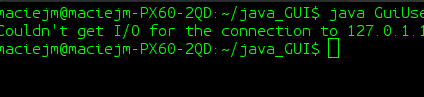
\includegraphics[width=0.4\hsize]{figures/IOError.png}}
		\caption{Input Output error from the server.}
	\end{figure}

	It means that the server is down and you need to contact the application administrator to get it up before you can run the game. If that has happened you will be presented with the following screen:

	\begin{figure}[htp]
		\centering
		\makebox{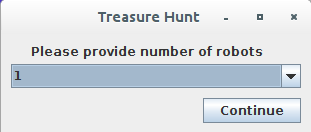
\includegraphics[width=0.4\hsize]{figures/App1.png}}
		\caption{Number of robots prompt.}
	\end{figure}

	This means that the application is ready to start playing the game. If you select the number of robots you should then be presented with the following screen:

	\begin{figure}[htp]
		\centering
		\makebox{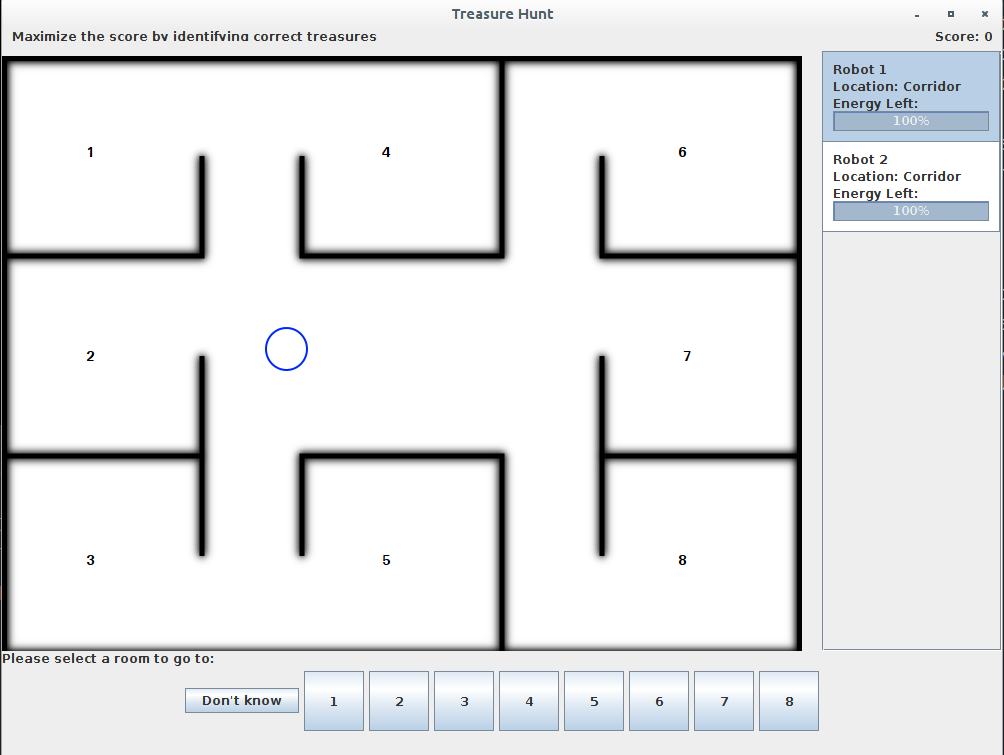
\includegraphics[width=0.4\hsize]{figures/finished.png}}
		\caption{Full GUI.}
	\end{figure}

	This is the UI interface from which you can play the game. Once you select a room a robot will engage in a conversation with you whether or not you wish to visit the room: \\
	\begin{figure}[htp]
		\centering
		\makebox{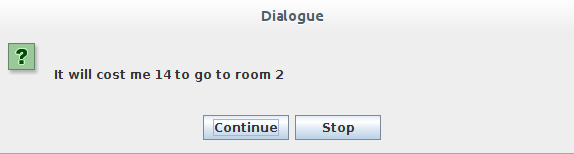
\includegraphics[width=0.4\hsize]{figures/App2.png}}
		\caption{Dialogue prompt}
	\end{figure}
	If so, the robot will set itself to a traveling state until it reaches that room. \\
	\begin{figure}[htp]
		\centering
		\makebox{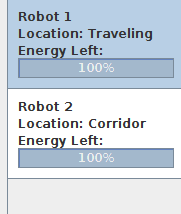
\includegraphics[width=0.3\hsize]{figures/App3.png}}
		\caption{Robot traveling.}
	\end{figure}
	You can also select another robot if you selected more than one robot to control at the start. If that's so please notice that the room that you sent your previous robot to will not be click-able. This just means you can choose each room once so choose wisely.
	\begin{figure}[htp]
		\centering
		\makebox{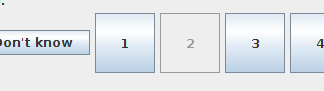
\includegraphics[width=0.3\hsize]{figures/App4.png}}
		\caption{Room no longer click-able.}
	\end{figure}
	Once the robot arrives to its destination. You will be prompted about the treasure footprint and colour that the robot discovered. You will be able to choose a treasure from a set of desired ones. These treasures will closely identify to the colour or footprint so you can make the decision now or take a picture.
	\begin{figure}[htp]
		\centering
		\makebox{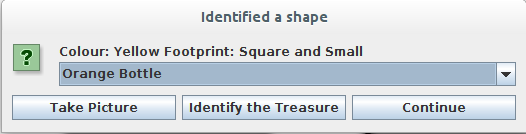
\includegraphics[width=0.3\hsize]{figures/App5.png}}
		\caption{Prompt regarding robot finding the treasure.}
	\end{figure}

	Before clicking identify the treasure you should always make sure that you select a treasure from the drop-down list first otherwise the first selection on that list will be carried out which would not be ideal. Remember that taking pictures costs so try to minimize the need to do so. For now take a picture for learning purposes.

	\begin{figure}[htp]
		\centering
		\makebox{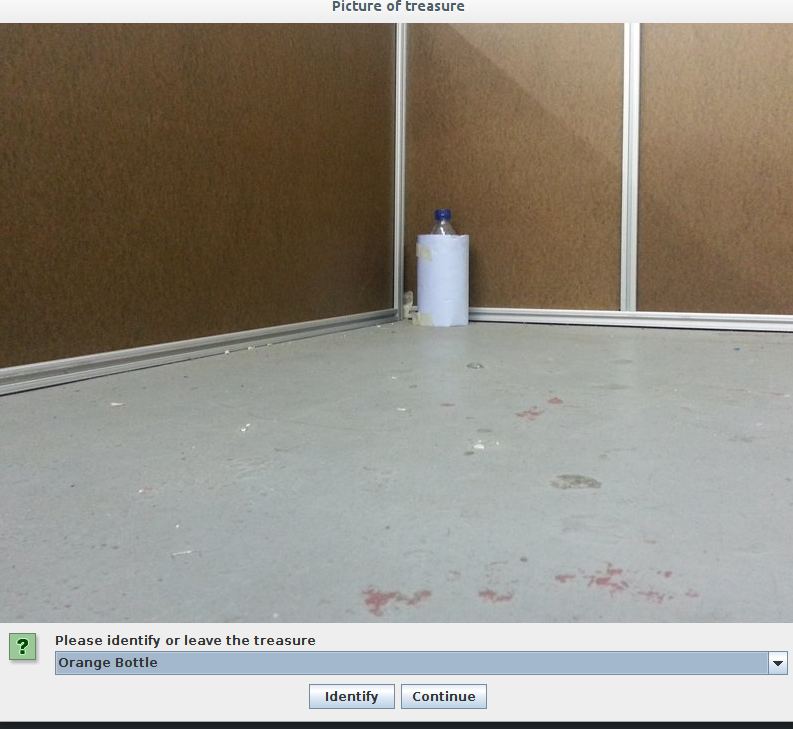
\includegraphics[width=0.3\hsize]{figures/App6.png}}
		\caption{Effect of taking a picture}
	\end{figure}

	You are now presented with a picture of the treasure and should be able to deduce what you are seeing but you can still press continue to forfeit the treasure. If you however identify and treasure you will receive a reply similar to this one:

	\begin{figure}[!htp]
		\centering
		\makebox{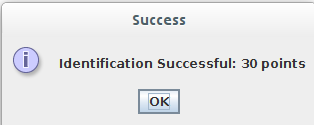
\includegraphics[width=0.3\hsize]{figures/App7.png}}
		\caption{Successful identification}
	\end{figure}

	Continue the previous steps and try to maximize the score as well as visit all the rooms. When you either visit all the rooms or the energy runs out from your robots you will finish the game. At that point you will receive the following type of message:
	\begin{figure}[htp]
		\centering
		\makebox{
\includegraphics[width=0.8\hsize]{figures/App8.png}}
		\caption{Game finished.}
	\end{figure}

	This will conclude the user guide for playing the game.

	\section{Admin Guide}
	This guide is aimed towards a person that has already set up the environment and looks to customize the program a little bit or start modifying it to their needs. It includes information on handling templates and how these templates are used in the program. It also says where to look for debugging tools in the software to ensure that there is a full coverage of information starting with the basics.
		\subsection{Templates}
		The GUI software boasts three templates in its system each of which contains information by which the program runs. You can edit each of those by a specific set of commands.\\
		\textbf{mapTimes template}: This is by far the most difficult template to get right but if eventually done it allows for customized cost creation for the robots. It is in a form of the first line containing the number of nodes in the matrix with the following lines being costs of x and y in the form of 'from' to 'to'. For a better understanding you can use the following figure:
		\begin{figure}[!htp]
		\centering
		\begin{tabular} {l}

			9 \\
			99 17 14 17 13 13 16 13 15 \\
			99 99 18 23 10 19 21 18 21 \\
			99 17 99 18 15 14 19 17 19 \\
			99 23 22 99 18 10 22 19 21 \\
			99 18 22 26 99 26 22 22 29 \\
			99 26 21 17 21 99 22 20 24 \\
			99 29 27 29 24 24 99 16 21 \\
			99 24 24 26 20 20 15 99 17 \\
			99 27 27 29 24 25 23 18 99 \\
		\end{tabular}
		\caption{Map Adjacency matrix}
		\end{figure}

		\textbf{DialogueText template}: This template is responsible for the type of questions you may want to ask your users when you present them with a GUI and allows for the dialogue between the robot and the user when a room is selected to go to to make sure that's what the user wants. This template follows a convention. The first line in the template defines the name of the template, the next lines until "SpecificRoom:" line are responsible for asking the users questions that relate to not being sure. Following the Specific room line are questions that you want to ask the user with regards to selecting a specific room. There is also built-in support for two reserver words that will be replaced with actual values in the environment. These values are £room£ and £cost£ both of which mean their implied meaning which is the room that the user wants to visit and the cost to get there. An example of the following template can be:

		\begin{figure}[!htp]
		\centering
		\begin{tabular} {l}
			DontKnow: \\
			Do you want me to go to room £room£ \\
			It will cost me £cost£ to go to room £room£ \\
			Are you sure? \\
			SpecificRoom: \\
			It will cost me £cost£ to go to room £room£ \\
			Are you sure? \\
		\end{tabular}
		\caption{Dialogue template}
		\end{figure}

		This template is currently used by the developed environment.
		\textbf{treasures template}: This template exists in two versions and follows a simple standard. That is the first line represents the number of rooms on a map. The hider uses this value to determine the number of treasures to disperse. The lines following this one are treasure descriptions each of which follows the same format. That is: \{Colour, Footprint, Points, What the treasure actually is, Filename\}. These values of comma separated and don't hold any parenthesis. If parenthesis will be used they will be treated as part of the treasure description. The filename is omitted in the template used by the GUI so whenever editing one make sure to change it in the GUI as well for compatibility reasons.

		\section{Running the application}
		The application is extremely easy to start on the environment that already supports it. To run the full stack, navigate to respectable folders of the implementation in the terminal and type the following commands to run the full system:
		\begin{itemize}
			\item \$ java Server 6009
			\item \$ roslaunch robot launch\_robot.launch
			\item \$ java Hider
			\item \$ java GuiUser
		\end{itemize}
		If the execution went correctly then the Server should produce a list of clients connected. Together it should connect TabUI, Hider and SimR. If you wish to debug at any point you can always use the Rviz package inside ROS. At the time of delivery it was left switched on so if you'd like to switch it off please use comment it out in the launch\_robot.launch file inside the Ros package robot.